%In the previous section each component of the system was modeled with differential and algebraic equations. The modeling format is such that every component takes some inputs, and from those calculates some states and some outputs which are used for the adjacent components. In order to make a complete non-linear model it is necessary to connect the inputs and outputs of the system. This section provides insight into how components are interfaced and collected into a complete non-linear state space form.

In the previous section each component of the system was modeled with differential and algebraic equations. The equations for each component generally require inputs from adjacent components, to generate outputs used for adjacent component. The aim of this section is to create a state space model which encapsulates all these interconnections. The model is expected to be non-linear as a direct result of the generally non-linear physics that describe thermodynamical systems. \cref{sec:mod_lin} will cover how the model is linearised.\\

A block diagram in \cref{fig:Block_diagram_inout} gives an overview of the system interface variables and states. In the diagram the component interface variables are split out to show which variables are used as inputs and outputs for each component. Some inputs to components are highlighted in red to signify that they are not found as outputs from a component. Steady State values (operating points) are used for these. The values are found by investigating a high-fidelity simulation of the system, provided by BITZER. Blue variables are outputs of components which are currently not used by the following component. Each component block also contains the names of the states they contain.

\begin{figure}[h!]
	\centering
	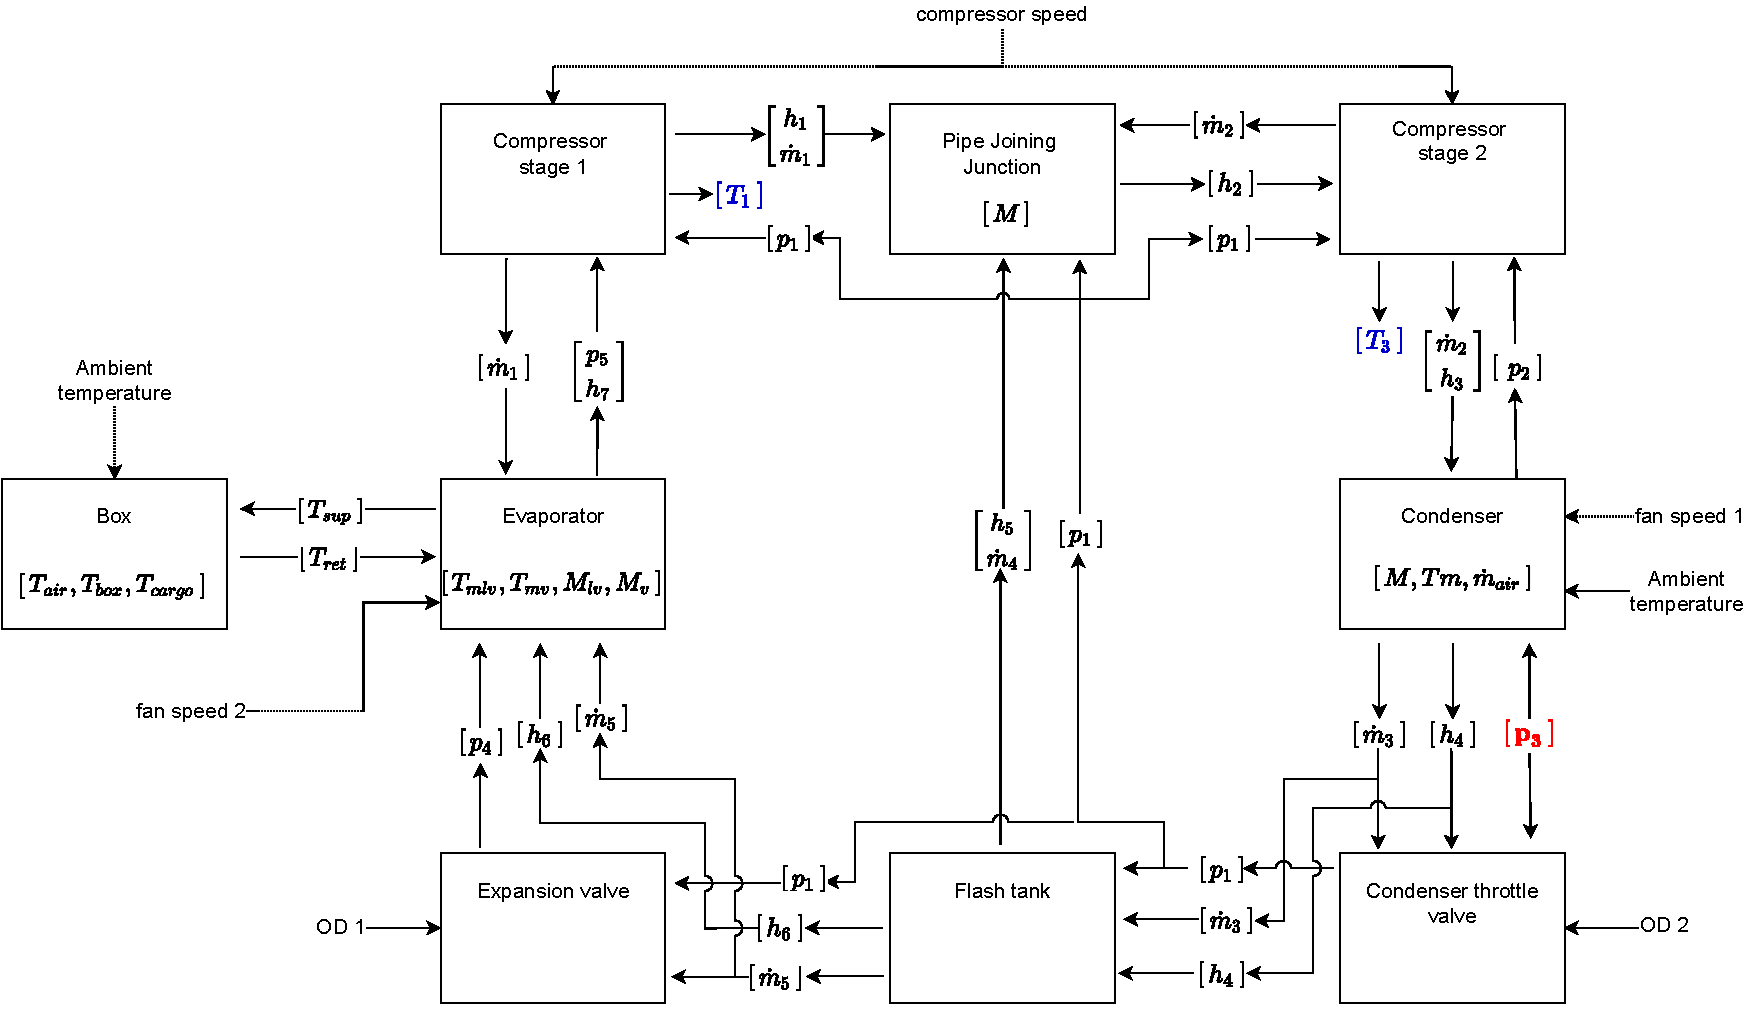
\includegraphics[width=1\textwidth]{Graphics/Block_Diagram_inout.pdf}
	\caption{Block diagram of input/output relationship of interface variables}
	\label{fig:Block_diagram_inout}
\end{figure}


\newpage

\subsubsection{State variables}

As described in \cref{sec:mod}, there is a large variance in dynamical speed across the system parameters. Therefore, the fast variables were defined algebraically, while the slow dynamics were modeled with differential equations. This modelling choice is valid since the fast variables rapidly settle to steady state values without oscillatory behavior. \\


The variables, which in \cref{sec:mod} were defined with differential equations are the system states. These are combined as a state vector $x$. The controlled inputs are likewise combined in the input vector $u$. These vectors are seen in \cref{eq:xu}.
%\begin{equation} \label{eq:xu} \renewcommand{\arraystretch}{2.4}
%	x = \begin{bmatrix}
%		M_{pjj}			\\				%pjj
%		M_{con} 		\\				%condenser
%		T_m 			\\				%condenser
%		\dot{m}_{air}	\\				%evaporator
%		T_{mlv}			\\				%evaporator
%		T_{mv}			\\				%evaporator
%		M_{lv}			\\				%evaporator
%		M_v				\\				%evaporator
%		T_{air}			\\				%box
%		T_{box}			\\				%box
%		T_{cargo}		\\				%box
%	\end{bmatrix} \;\;\;\;\;\;\;\;\;
%	u = \begin{bmatrix}
%		\Theta_1			\\				%pjj
%		\Theta_2 		\\				%condenser
%		U_{fan_1}			\\				%condenser
%		U_{fan_2}	\\				%evaporator
%		\omega			\\				%evaporator
%\end{bmatrix}
%\end{equation}
\begin{equation} \label{eq:xu} \renewcommand{\arraystretch}{2.4}
	x = \begin{bmatrix}
		M_{pjj}				&		%pjj
		M_{con} 			&		%condenser
		T_m 				&		%condenser
		\dot{m}_{air}		&		%evaporator
		T_{mlv}				&		%evaporator
		T_{mv}				&		%evaporator
		M_{lv}				&		%evaporator
		M_v					&		%evaporator
		T_{air}				&		%box
		T_{box}				&		%box
		T_{cargo}			&		%box
	\end{bmatrix}^T ,  \;\
	u = \begin{bmatrix}
		\Theta_1			&			%pjj
		\Theta_2 			&			%condenser
		U_{fan_1}			&			%condenser
		U_{fan_2}			&			%evaporator
		\omega							%evaporator
	\end{bmatrix}^T
\end{equation}
We define a function $f(x,u)$ as a vector of the state derivatives:
% F: States
% ------------------------------------

\begin{equation} \label{eq:f_noSub} \renewcommand{\arraystretch}{2.4}
	f(x,u) =  \dfrac{d}{dt} \begin{bmatrix}
		M_{pjj}			\\				%pjj
		M_{con} 		\\				%condenser
		T_m 			\\				%condenser
		\dot{m}_{air}	\\				%evaporator
		T_{mlv}			\\				%evaporator
		T_{mv}			\\				%evaporator
		M_{lv}			\\				%evaporator
		M_v				\\				%evaporator
		T_{air}			\\				%box
		T_{box}			\\				%box
		T_{cargo}		\\				%box

	\end{bmatrix}
	=
	\begin{bmatrix}
		\dot{m}_1 + \dot{m}_4 - \dot{m}_2 \\										%pjj
		\dot{m}_{2} - \dot{m}_{3}	\\												%condenser
		\dfrac{Q_{rm} - Q_{ma}}{M_m \cdot Cp_m} \\									%condenser
		\dfrac{\bar{\dot{m}}_{air}  - \dot{m}_{air}} {10s}		\\					%evaporator
		\dfrac{Q_{aml}-Q_{ml} + Q_{mvml}}{M_m \cdot Cp_m \cdot \sigma}        \\	%evaporator
		\dfrac{Q_{amv} - Q_{mv} - Q_{mvml}}{M_m \cdot Cp_m \cdot (1- \sigma)}	\\	%evaporator
		\dot{m}_{5} - \dot{m}_{dew}		\\											%evaporator
		\dot{m}_{dew} - \dot{m}_{1}	\\												%evaporator
		\dfrac{Q_{ca} + Q_{ba} + Q_{fan} -Q_{cool}}{M_{air} \cdot Cp_{air}} \\		%box
		\dfrac{Q_{amb} - Q_{ba}}{M_{box} \cdot Cp_{box}} \\							%box
		\dfrac{-Q_{ca}}{M_{cargo} \cdot Cp_{cargo}}									%box
	\end{bmatrix}
\end{equation}

\cref{eq:f_noSub} does not immediately look like a typical set of ODE's. However, all the variables on the right most side of the equation, can be substituted with the algebraic equations from the modelling section. Once no more substitutions can be made $f(x,u)$ will be a function of the system states, inputs and disturbance. The function $f(x,u)$ is thus the non-linear model of the system. The model contains 11 states, 5 control inputs and 1 disturbance. Writing out the full equation is infeasible due to the sheer size of expressions when substitution is performed.

One issue encountered when observing the behavior of the non-linear model concerned the state $M_v$. When simulating the non-linear system model with inputs held constant at the operating point the derivative of the state $M_v$ converges to a non-zero constant, which makes the state integrate towards infinity. This error is considered as a numeric error. From a physical standpoint it does not make sense for vapor mass to accumulate indefinitely and thus a simple fix is used to omit it: The constant value of the derivative was subtracted. \\

In details, the constant was discovered to be a function of the compressor speed. The value subtracted is thus also a function of the compressor speed. This removed the integrating effect, but may imply that some numerical errors were present in the non-linear model. Further investegations of the phenomenon were performed but did not reveal the origin of the error. No further actions were thus taken.

%The control inputs are:

%\begin{center}
%	\begin{tabular}{l p{10cm}}
%		$ \Theta_1 $  & The valve opening degree of the \\
%		$ \Theta_2 $  & The valve opening degree of the \\
%		$ U_{fan_1} $ & The condenser fan speed         \\
%		$ U_{fan_2} $ & The evaporator fan speed        \\
%		$ \omega $    & The compressor speed
%	\end{tabular}
%\end{center}

%The disturbance is:

%\begin{center}
%	\begin{tabular}{l p{10cm}}
%		$ T_{ambi} $  & The ambient air temperature
%	\end{tabular}
%\end{center}